\documentclass[11pt]{article}
\pdfoutput=1

\usepackage{amsmath,amssymb}
\usepackage{hyperref}
\usepackage{graphicx}
\usepackage[small]{caption}
\usepackage[svgnames,dvipsnames,x11names,table]{xcolor}
\usepackage{booktabs}
\usepackage{microtype}
\usepackage[framemethod=default]{mdframed}

\setlength{\textwidth}{460pt}
\setlength{\topmargin}{-1.2cm}
\setlength{\textheight}{640pt}
\setlength{\oddsidemargin}{10pt}
\linespread{1.1}

\numberwithin{equation}{section}

\newmdenv[skipabove=7pt,skipbelow=7pt,rightline=false,leftline=false,
topline=false,bottomline=false,backgroundcolor=blue!6,linecolor=blue!40,
innerleftmargin=6pt,innerrightmargin=6pt,innertopmargin=5pt,innerbottommargin=5pt,
leftmargin=0cm,rightmargin=0cm,linewidth=3pt]{IntuitionBox}

\newmdenv[skipabove=7pt,skipbelow=10pt,rightline=false,leftline=false,
topline=false,bottomline=false,backgroundcolor=green!6,linecolor=green!30!black,
innerleftmargin=6pt,innerrightmargin=6pt,innertopmargin=5pt,innerbottommargin=5pt,
leftmargin=0cm,rightmargin=0cm,linewidth=3pt]{TakeawayBox}

\title{BTC Daily Realized Volatility:\\ Weekly Seasonality and In-Sample HAR Fits}
\author{}
\date{2026-10-26}

\begin{document}
\maketitle

\noindent\textbf{Data.} BTCUSDT daily log realized volatility $\log RV_t^{(d)}$ from 5-minute log returns $r_t = p(t) - p(t-\Delta)$, days starting 00:00 UTC ($\tau = 0$), 2022-01-02 to 2026-09-30, $n = 1733$ consecutive days with no gaps. Produced by \texttt{compute\_rv.py}. The spectral results (Sections 1--4) come from \texttt{periodogram\_findings.py}; the HAR fits (Section 5) from \texttt{compute\_rv.py}.

\noindent\textbf{Scope: everything here is in-sample.} The weekday means and the HAR coefficients are estimated on the full sample and evaluated on the same days. That is appropriate for describing the data, but it is not a forecast test: out-of-sample evaluation (rolling-origin forecasts from 2024-01-01, with weekday effects estimated on each training window only) is the next phase.

\begin{TakeawayBox}
\textbf{Summary.}
\begin{enumerate}
\item The only clear cycle is \textbf{weekly}. It shows up as peaks at periods of 7, 3.5 and 2.33 days; the last two are harmonics of the week, not separate cycles.
\item The weekly cycle is a \textbf{weekend dip}: Saturday is about 0.47 below the mean in log RV (roughly 37\% lower RV), Sunday about 0.24 below, and the five weekdays are nearly flat. Weekday means explain \textbf{22\%} of the variance of log RV.
\item Removing weekday means removes all three weekly peaks. What is left at long periods is a rising background (long memory) with no peak that survives a correction for the number of frequencies tested, or a smoothed (Welch) spectrum.
\item \textbf{In a HAR model, the weekly cycle matters for both fit and coefficients.} Adding weekday dummies raises the in-sample $R^2$ from 0.43 to 0.65 and cuts the residual standard deviation from 0.37 to 0.29. Without them, the daily coefficient is understated (0.39 vs 0.48) and the monthly one looks insignificant ($t = 1.2$ vs $2.3$).
\end{enumerate}
\end{TakeawayBox}

\section{The periodogram}

For the demeaned series $x_t = \log RV_t - \overline{\log RV}$, $t = 0,\dots,n-1$, the periodogram at the Fourier frequencies $f_k = k/n$ (cycles per day) is
\begin{equation}
I(f_k) = \frac{1}{n}\Bigl|\sum_{t=0}^{n-1} x_t\, e^{-2\pi i f_k t}\Bigr|^2 ,
\end{equation}
plotted against period $1/f_k$ for periods of 2 to 90 days. Two properties matter for reading it:
\begin{itemize}
\item \textbf{Each ordinate is noisy.} For a stationary series, $I(f_k)/S(f_k)$ is approximately exponential with mean 1, where $S$ is the true spectrum: the real and imaginary parts of the Fourier sum are approximately independent Gaussians of equal variance, so $2I/S \sim \chi^2_2$. Its standard deviation equals its mean, at every frequency and for every $n$. A single ordinate 3 times the local level happens with probability $e^{-3} \approx 0.05$ by chance, so isolated spikes of that size are expected.
\item \textbf{Resolution is coarse at long periods.} Frequencies are spaced $1/n$ apart, so neighbouring periods near 90 days are $n/19 \approx 91$ and $n/20 \approx 87$ days. Peaks between 30 and 90 days cannot be located precisely.
\end{itemize}

\begin{figure}[h]
\centering
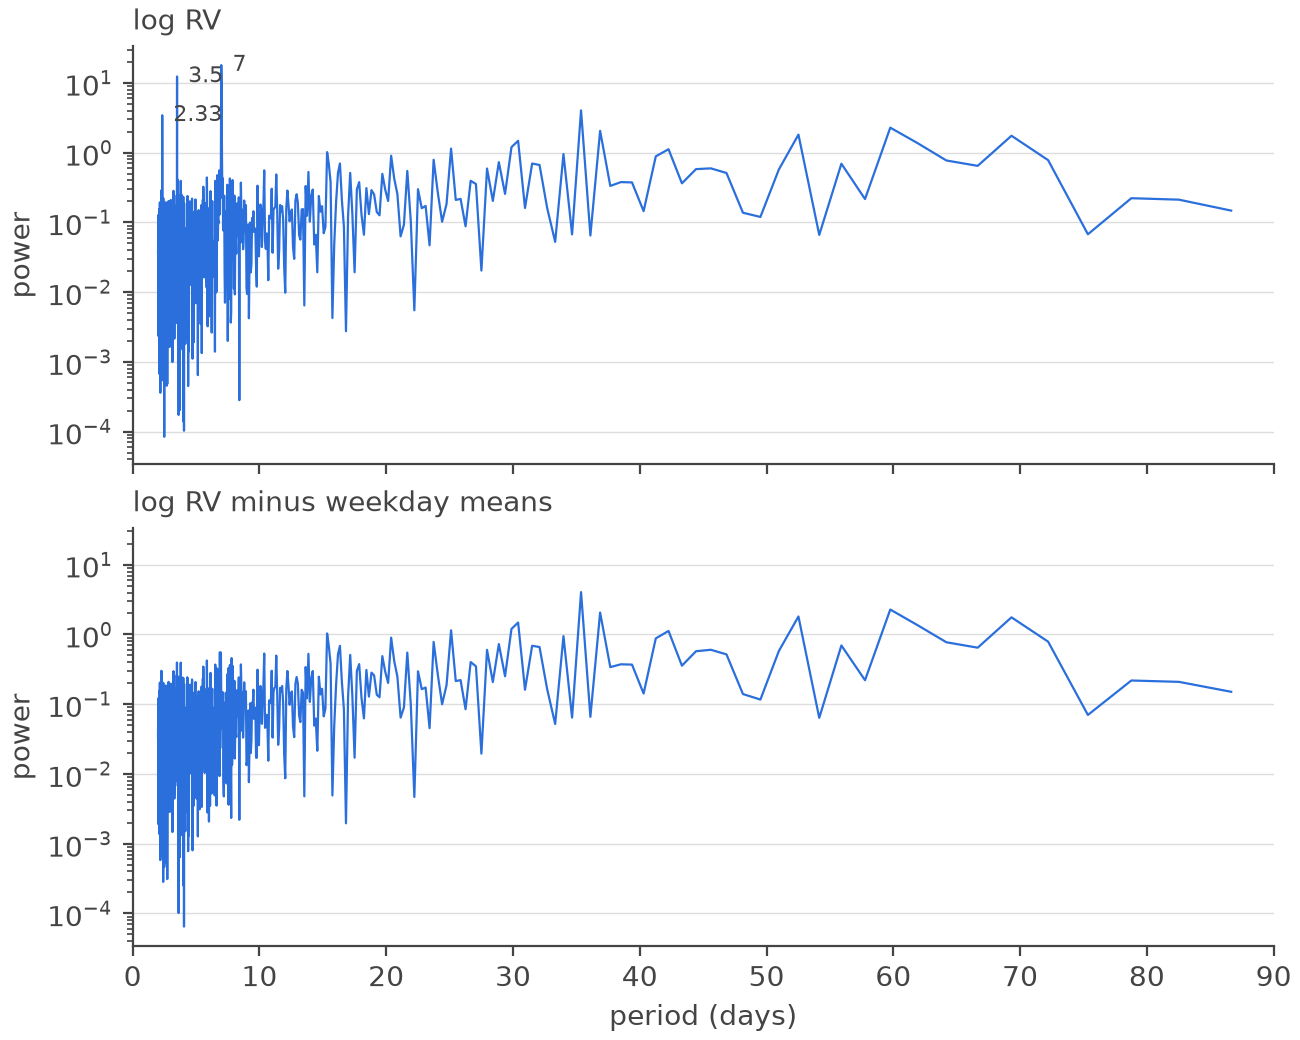
\includegraphics[width=0.92\textwidth]{periodogram_before_after.png}
\caption{Periodogram of log RV (top) and of log RV after subtracting the mean for each day of the week (bottom). Log scale. The three weekly peaks are labelled in the top panel and vanish in the bottom one; the rest of the spectrum is unchanged.}
\label{fig:periodogram}
\end{figure}

The weekday means used here and below are computed over the whole sample. That suits a description of the data; a forecasting model must estimate them on its training window only (Section~5 does this implicitly with dummies).

\section{The weekly cycle and its harmonics}

The top panel of Figure~\ref{fig:periodogram} has three spikes far above the background:

\begin{center}
\begin{tabular}{lccc}
\toprule
period (days) & 7 & 3.5 & 2.33 \\
cycles per week $k$ & 1 & 2 & 3 \\
\midrule
power, log RV & 18.03 & 12.37 & 3.44 \\
power, after removing weekday means & 0.118 & 0.027 & 0.029 \\
\bottomrule
\end{tabular}
\end{center}

The background near these periods is about 0.1, so the raw peaks are 30 to 180 times the background. Removing weekday means brings all three back to background level.

\subsection{Why the harmonics appear}

Any pattern that repeats every 7 days can be written exactly as a sum of sines at $k/7$ cycles per day, i.e.\ at periods $7/k$. With daily data only $k = 1, 2, 3$ are distinct: the shortest observable period is 2 days (Nyquist), and $k = 4, 5, 6$ alias onto $3, 2, 1$. So a weekly pattern of \emph{any} shape lives entirely at periods 7, 3.5 and 2.33 days.

\begin{IntuitionBox}
\textbf{Intuition.} The periodogram asks, frequency by frequency, how well a sine of that period lines up with the data. A sine whose period does not divide the week drifts against the calendar, so it matches the weekend dip in some weeks and clashes with it in others, and the matches cancel. A sine with period 3.5 or 2.33 days completes exactly 2 or 3 cycles per week, sits at the same place relative to the weekdays every week, and its match accumulates.

Whether those harmonics actually carry power depends on the \emph{shape} of the weekly pattern. A smooth sine-shaped week would give a single peak at 7 days. A flat Monday--Friday followed by a sharp two-day drop cannot be built from one sine per week; the faster sines are needed to sharpen the drop and flatten the weekdays, so they show up as peaks.
\end{IntuitionBox}

\subsection{The weekday profile}

\begin{figure}[h]
\centering
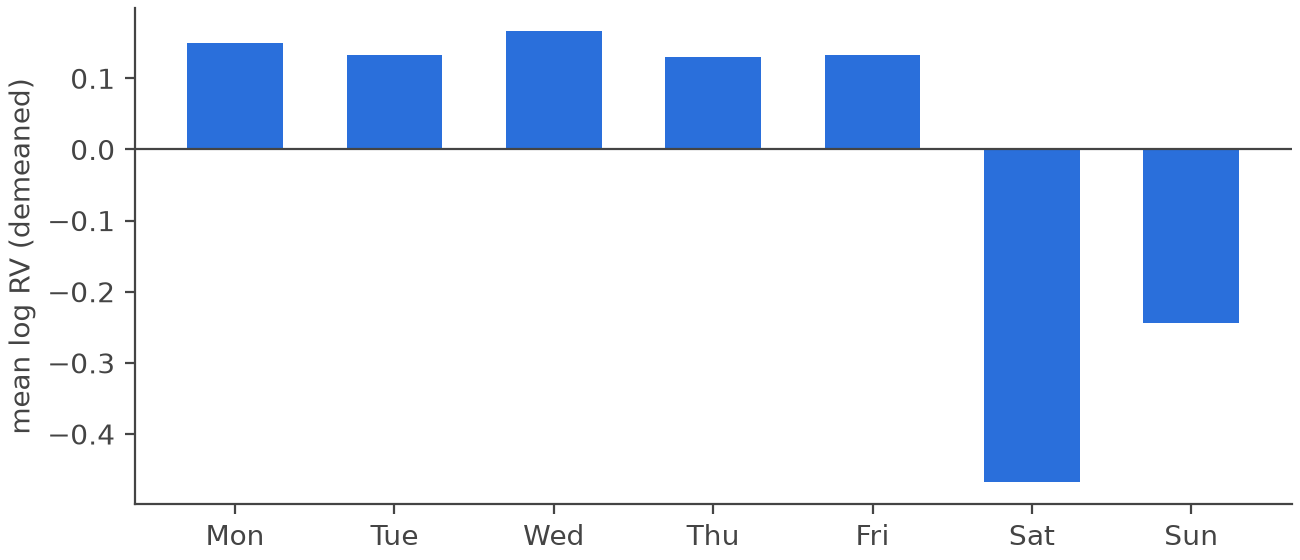
\includegraphics[width=0.75\textwidth]{periodogram_weekday.png}
\caption{Mean of demeaned log RV by day of the week (UTC).}
\label{fig:weekday}
\end{figure}

Figure~\ref{fig:weekday} shows the profile directly. Monday to Friday sit between $+0.13$ and $+0.17$; Saturday is $-0.47$ and Sunday $-0.24$. Sunday is less quiet than Saturday, plausibly because the end of the UTC Sunday overlaps the start of the trading week (CME bitcoin futures reopen Sunday evening US time, and Asian markets open early Monday local time).

The relative power that this profile puts at the three harmonics matches the periodogram's ordering, and is close to an idealised ``low on Saturday and Sunday, flat otherwise'' block:

\begin{center}
\begin{tabular}{lccc}
\toprule
relative power at period & 7 & 3.5 & 2.33 \\
\midrule
empirical weekday profile & 1.00 & 0.45 & 0.13 \\
idealised weekend block & 1.00 & 0.48 & 0.06 \\
\bottomrule
\end{tabular}
\end{center}

\section{Long periods (20--90 days)}

After removing weekday means, the six largest ordinates with periods of at least 20 days are below. ``Ratio'' is the ordinate divided by the mean of its neighbours (excluding the immediately adjacent ones), and $P$ is $e^{-\text{ratio}}$, the chance of a ratio that large at one frequency under no periodicity.

\begin{center}
\begin{tabular}{cccc}
\toprule
period (days) & power & ratio to local background & $P$ (single frequency) \\
\midrule
35.4 & 4.05 & 7.0 & 0.001 \\
59.8 & 2.28 & 3.1 & 0.044 \\
36.9 & 2.06 & 2.5 & 0.080 \\
52.5 & 1.81 & 2.5 & 0.083 \\
69.3 & 1.76 & 2.7 & 0.068 \\
30.4 & 1.48 & 3.4 & 0.032 \\
\bottomrule
\end{tabular}
\end{center}

There are 67 Fourier frequencies with periods between 20 and 90 days. Testing all of them, the chance that at least one reaches $P = 0.001$ is about $1 - 0.999^{67} \approx 0.065$, and several reaching $P \approx 0.05$ is expected.

These $P$ values are slightly optimistic: $e^{-\text{ratio}}$ treats the local background as known exactly, whereas it is itself estimated from a few neighbouring ordinates, each with the same exponential scatter. Accounting for that would make every candidate below weaker, not stronger. So:
\begin{itemize}
\item \textbf{35.4 days} is the only candidate, and it is borderline (family-wise $p \approx 0.07$, before the correction above). It is not a multiple of anything obvious; its neighbour at 36.9 days is also somewhat elevated, which could mean a broad bump rather than a sharp cycle. In the Welch spectrum (364-day Hann segments, 50\% overlap; panel in \texttt{rv\_daily\_tau0.png}), which averages several segment periodograms and so reduces the scatter, it appears only as a bump of about a factor of 2 within the remaining noise, not as a line above the background.
\item \textbf{30.4 days} equals the average calendar month ($365.25/12$), which makes it a natural hypothesis (for example monthly futures and options expiries). On its own the periodogram gives no real evidence for it ($P = 0.03$ at one of 67 frequencies). A direct test, such as an expiry-day dummy in the RV regression, would be more informative than the spectrum.
\item The rest is the \textbf{rising background}: power grows towards longer periods, the frequency-domain view of the slowly decaying autocorrelation (long memory, or the HAR-type persistence Corsi models).
\end{itemize}

\section{Effect on the autocorrelation}

The weekly cycle also explains the spikes at lags 7, 14, 21, \dots\ in the autocorrelation of log RV. After removing weekday means the autocorrelation decays smoothly: it falls at multiples of 7 (the weekly echo is gone) and rises at every other lag, because the weekly swings no longer act as noise:

\begin{center}
\begin{tabular}{lccccccc}
\toprule
lag (days) & 1 & 5 & 7 & 14 & 22 & 30 & 66 \\
\midrule
log RV & 0.61 & 0.30 & 0.57 & 0.46 & 0.25 & 0.13 & 0.01 \\
log RV minus weekday means & 0.72 & 0.48 & 0.45 & 0.31 & 0.26 & 0.26 & 0.14 \\
\bottomrule
\end{tabular}
\end{center}

\noindent Single lags of the raw series can mislead: lag 66 (0.01) falls in a trough between weekly peaks at lags 63 and 70 (both about 0.34). Those peaks are consistent with the weekly share of the variance plus the remaining memory, $0.22 + 0.78 \times 0.14 \approx 0.33$.

\section{In-sample HAR fits}

\subsection{Model}

The log-HAR model (Corsi, 2009, in logs) with windows $(1, w, m)$ forecasts the next day's log RV, $y_{t+1}$, from averages of log RV up to and including day $t$:
\begin{equation}
y_{t+1} = c + \beta_d\, y_t + \beta_w\, \bar y^{(w)}_t + \beta_m\, \bar y^{(m)}_t + \sum_{j \neq \text{Mon}} \gamma_j\, D_j(t+1) + \varepsilon_{t+1},
\qquad \bar y^{(h)}_t = \frac1h \sum_{i=0}^{h-1} y_{t-i},
\end{equation}
where $D_j(t+1)$ indicates that the \emph{target} day $t+1$ is weekday $j$ (Monday is the baseline). The target day's weekday is known at the forecast origin, so the dummies use no future information. Since day $t$'s weekday is fixed by day $t+1$'s, one set of target-day dummies also absorbs the weekly cycle carried by the regressors.

All fits use the same 1,703 days (2022-01-31 to 2026-09-29: the 30-day window and the next-day target remove 30 of the 1,733), so their $R^2$ values are directly comparable when the target is the same. Coefficients are OLS; standard errors are Newey--West (Bartlett kernel) with 7 lags, from the rule $\lfloor 4 (n/100)^{2/9} \rfloor$.

\subsection{Results}

\begin{center}
\small
\begin{tabular}{lcccc}
\toprule
 & plain HAR & HAR + weekday dummies & \multicolumn{2}{c}{HAR on weekday-adjusted series} \\
 & (1, 7, 30) & (1, 7, 30) & (1, 7, 30) & (1, 5, 22) \\
target & $\log RV$ & $\log RV$ & $\log RV_{\text{adj}}$ & $\log RV_{\text{adj}}$ \\
\midrule
$c$ & $-0.517$ & $-0.169$ (Monday) & $-0.440$ & $-0.498$ \\
$\beta_d$ & 0.388 (15.6) & \textbf{0.485} (15.1) & 0.485 (15.1) & 0.460 (14.5) \\
$\beta_w$ & 0.427 (10.4) & \textbf{0.312} (7.4) & 0.313 (7.4) & 0.306 (7.5) \\
$\beta_m$ & 0.051 (1.2) & \textbf{0.089} (2.3) & 0.089 (2.3) & 0.105 (2.8) \\
\midrule
$R^2$ & 0.428 & \textbf{0.648} & $0.544^{*}$ & $0.543^{*}$ \\
residual s.d. & 0.373 & \textbf{0.293} & 0.293 & 0.293 \\
\bottomrule
\end{tabular}
\end{center}
\noindent Newey--West $t$-statistics in parentheses. $^{*}R^2$ on the weekday-adjusted target, whose variance is 22\% smaller than that of $\log RV$; not comparable with the first two columns.

\noindent Weekday dummies (shift relative to Monday, given the same HAR inputs): Tue $-0.208$, Wed $-0.169$, Thu $-0.221$, Fri $-0.205$, Sat $-0.810$, Sun $-0.285$; all $|t| > 6$.

\subsection{Interpretation}

\begin{enumerate}
\item \textbf{Modelling the weekly cycle is a large gain.} On the same target and the same days, six calendar dummies raise $R^2$ from 0.428 to 0.648 and reduce the residual standard deviation from 0.373 to 0.293, about 21\% smaller errors.

\item \textbf{Dummies and pre-adjustment give the same model.} The HAR coefficients from the dummies fit and from the fit on the weekday-adjusted series agree to four decimals, with the same residual standard deviation (Frisch--Waugh--Lovell: the dummies remove each variable's weekday means within the regression). The $R^2$ values differ only because the targets have different variances: $0.293^2/(1-0.648) \approx 0.244$, the variance of $\log RV$, against $0.293^2/(1-0.544) \approx 0.188$. The intercepts differ only by baseline: Monday's $-0.169$ plus the average of the seven weekday shifts (Monday's being zero), $-0.271$, gives $-0.440$. The agreement is close but not exact by construction (weekday means from 1,733 days vs a fit on 1,703; demeaning the averages vs averaging an adjusted series).

\item \textbf{Ignoring the weekly cycle distorts the HAR coefficients.} Yesterday's value carries the weekday swing, a misleading signal around weekends, while the 7-day average contains one of each weekday and cancels it. The plain fit therefore moves weight from $\beta_d$ (0.39 instead of 0.48) to $\beta_w$ (0.43 instead of 0.31), and $\beta_m$ loses significance ($t = 1.2$ instead of $2.3$). A HAR model fitted to crypto RV without seasonal adjustment understates daily and monthly persistence.

\item \textbf{The dummies are conditional corrections, not weekday means.} All six are negative because Monday's inputs contain the quiet weekend, so HAR alone under-forecasts Monday most. Saturday's shift ($-0.81$) exceeds the raw Saturday dip ($-0.47$ against the mean) because Friday's busy inputs push the HAR forecast up. They should not be read as ``Saturday is 0.81 quieter''.

\item \textbf{Horizons.} Once the weekly cycle is handled, the calendar-day horizons (1, 7, 30) and the equity horizons (1, 5, 22) fit almost identically in-sample ($R^2$ 0.544 vs 0.543 on the adjusted target).
\end{enumerate}

\section{Implications for modelling}

\begin{TakeawayBox}
\begin{itemize}
\item Handle the weekly cycle explicitly inside the HAR model. Day-of-week dummies for the target day are equivalent in-sample to pre-adjusting the series (Section 5), and are the choice for forecasting: they give forecasts on the original scale, and the weekday effects are estimated on the training window automatically. Sines and cosines at $k = 1, 2, 3$ cycles per week would be equivalent to the dummies.
\item Do not add a separate 3.5-day or 2.33-day term; they are part of the weekly pattern.
\item The HAR horizons were set for equity markets (5 and 22 trading days). For a market that trades every day, 7 and 30 calendar days are the natural weekly and monthly horizons; in-sample the choice barely matters once the weekly cycle is modelled, so it should be decided on forecast performance.
\item There is no evidence for any cycle longer than a week: the 35.4-day candidate does not stand out in the Welch spectrum.
\item All of the above is in-sample. Whether the gain from the weekday dummies holds in out-of-sample forecasts is the next test.
\end{itemize}
\end{TakeawayBox}

\section*{Reference}

\noindent Corsi, F. (2009). A simple approximate long-memory model of realized volatility. \emph{Journal of Financial Econometrics}, 7(2), 174--196.

\end{document}
